\section{Portable Batch System - PBS}
%\label{cap:pbs}

Desenvolvido para fornecer processamento em lote, ao contrário de colocar um processo em segundo plano, o processamento em lote do PBS abrange o escalonamento de múltiplas tarefas conforme as políticas do RMS. Cada tarefa pode conter inúmeros processos. Essas tarefas podem ser direcionadas para rotear processos através de nós em uma rede. É possível a reserva de recursos para determinada tarefa antes do início da sua execução \cite{Bayucan1998a}.

\section{PBS - Cliente}

Comandos devem estar de acordo com a especificação POSIX.15. É possível especificar mais de uma operação na linha de comando onde essas serão interpretadas uma de cada vez. A geração de um erro de operando em determinado servidor será colocado na saída de erro padrão. O comando continua executando demais operandos. Sendo que o recebimento de qualquer erro por qualquer operando, resultará em um \emph{status} final maior que zero.

\section{PBS - Servidor}

O servidor principal tem como foco principal a comunicação dos clientes e gerenciar as tarefas. O servidor é o coração do sistema e suas principais responsabilidades são \cite{Bayucan1998a}:

\begin{itemize}
	\item possuir e controlar tarefas em lotes.
	\item possuir e controlar filas.
	\item recuperar estado de tarefas e filas.
	\item executar serviços em nome de clientes baseado em um serviço de requisição de lote.
	\item executar serviços adiados em nome de tarefas baseadas em eventos externos.
	\item iniciar seleção de tarefas para execução baseado em um grupo local definido de políticas de regras.
	\item estabelecer recursos reservados e usar limites para tarefas iniciadas no local de execução.
	\item colocar uma tarefa de lote em execução e monitorar seu progresso.
	\item executar o processamento e a limpeza de tarefas.
\end{itemize}

\section{Processo de Escalonamento}

O processo de escalonamento se caracteriza por uma escolha que elege qual tarefa será executada. Para isto, esta tarefa deve constar em uma fila de execução.

O PBS fornece um programa separado como um processo de seleção que maximiza a flexibilidade na implementação das políticas locais. O escalonador comunica-se com o servidor via um \emph{socket} IPC. Desta forma é possível possuir escalonador e servidor em diferentes nós.

Para cumprir seu papel de gerenciador de recursos, o escalonador se comunica com outro processo chamado \emph{Machine Oriented Mineserver} (MOM). Assim é possível recuperar informações sobre a carga do sistema do nó. Nestas informações podem conter detalhes do uso de memória, carga de CPU, entre outras. Esta relação entre PBS, o escalonador e o MOM é demostrado na figura~\ref{fig:Pbs_MOM} \cite{Bayucan1998}.

\begin{center}
	\begin{enumerate}
		\item Evento aviso o servidor para iniciar um ciclo de escalonamento.
		\item Servidor envia comando de escalonamento para Escalonador.
		\item Escalonador requisita informação de recursos do MOM.
		\item MOM retorna informações solicitadas.
		\item Escalonador requisita informações do servidor.
		\item Servidor envia informações de \emph{status} da tarefa para o escalonador. Escalonador realiza política para executar a tarefa.
		\item Escalonador envia solicitação de execução para o servidor.
		\item Servidor envia tarefa para o MOM executar.
	\end{enumerate}
\end{center}

\begin{figure}[htb]
\begin{center}
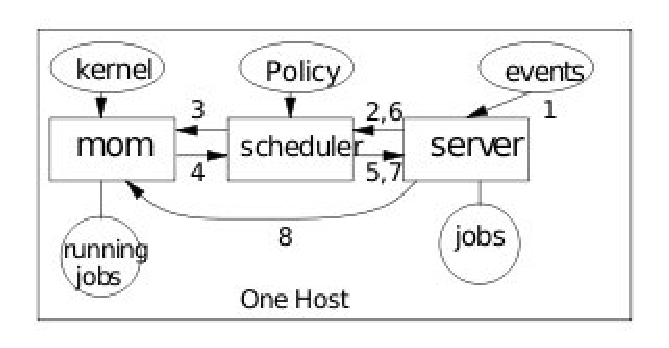
\includegraphics[scale=0.9]{./img/PbsMom.eps}
\caption{Escalonamento em um nó}
\label{fig:Pbs_MOM}
Fonte: \cite{Bayucan1998}
\end{center}
\end{figure}

Um ponto negativo no PBS é o fato deste ter um servidor centralizando, onde uma pane neste nó, afetaria o sistema por inteiro.

Para acesso as funcionalidades que o PBS oferece são fornecidas duas maneiras, um conjunto de \emph{scripts} de linha de comando e uma biblioteca de programação. A biblioteca escrita na linguagem C denominada \emph{Batch Interface Library} (IFL).